\documentclass{article}
\usepackage{graphicx}%вставка картинок
\usepackage{float}%"Плавающие" картинки
\newcommand{\RomanNumeralCaps}[1]
    {\MakeUppercase{\romannumeral #1}}
\linespread{0.87}%интервал между абзацами
\setcounter{page}{264}
\usepackage{multicol}%подключение колонн
\usepackage[top=2cm,bottom=2cm,left=2cm,right=2cm]{geometry}
\setlength{\columnsep}{0.6cm}%расстояние между колоннами
\begin{document}
\fontsize{10}{14}\selectfont%размер шрифта
\begin{multicols}{2}
\begin{itemize}
    \item schemes for the functioning of a hybrid intelligent
computer system, providing the possibility of semantic compatibility and sharing with other solutions at
industrial enterprises in the context of the Industry
4.0 concept [6];\vspace{-5pt}
\item algorithms for the synthesis of control feedback
based on the use of neuroregulators;\vspace{-5pt}
\item method of adaptive control of automated production
systems in the presence of external control influences;\vspace{-5pt}
\item software support for intelligent systems based on
adaptation algorithms and the proposed method in
real time.
\end{itemize}\vspace{-7pt}\par
The results provide a new constructive approach to
the formalization of the technological cycle, based on
the use of open semantic technologies for the design
of intelligent systems, and the synthesis of feedback on
the management of the production process using neural
network modeling, which allows to:
\begin{itemize}
\item develop hybrid intelligent computer systems designed to solve problems of adapting the management of complex technical systems, in particular, the
technological production cycle;\vspace{-5pt}
\item ensure integration and semantic compatibility of the
components of the control system model with other
intelligent systems;\vspace{-5pt}
\item search for optimal parameters for adapting control
and stabilizing controlled variables of technological
operations in specified ranges of permissible values.
\end{itemize}\par\vspace{-7pt}
The described tools make it possible to create flexible
intelligent computer control adaptation systems (CCAS),
which are a set of semantically compatible and easily
replaceable components depending on the range of tasks
being solved.\par
The interaction of the system and its corresponding
solvers with the control rack of the automated technological system is carried out using means of software and
hardware interface of production.
\begin{center}
\RomanNumeralCaps{3.} Constructing components of a multi-level control
system model in conditions of incomplete information
\end{center}\vspace{-5pt}\par
Optimization of the parameters of the technological
cycle of automated production requires the development
of effective control adaptation algorithms and methods
for constructing neuroregulators that stabilize the parameters of technological operations, taking into account
current information about the functioning of the object
of study, random disturbances and external control influences, which are recorded during the operation of the
control system controller and stored at the control rack
automated control system (ACS) for the technological
process (TP).\par
The structural diagram of the interaction of the components of the intelligent control adaptation system is
presented in figure 1. A formal description of the control
object is carried out based on the use of the ontology
of the “probabilistic technological production processes”
subject area. When implementing this approach, formalized knowledge is used to describe technological processes with probabilistic characteristics of technological
operations and model technological processes.\vspace{0.3cm}
\begin{figure}[H]
    \centering
    \includegraphics[width=8.5cm]{1.png}
 \caption{{\small Diagram of interaction of the components of the intelligent
control adaptation system}}
\end{figure}
The formalization used is based on the scientific research of the authors in the field of simulation modeling
of complex technical systems and implies the use of
libraries of simulator units of technological operations
integrated into the OSTIS ecosystem on the principles
of semantic compatibility [7].\par
When the characteristics of technological operations
of a control object are highly non-stationary, simulation
models, neuroregulators and multi-step learning algorithms with better dynamic properties are used to build
multi-level mathematical models.\par
As follows from the interaction diagram of the system
components, the formation of control feedback comes
down to the search for control adaptation that satisfies user-specified criteria, carried out according to the
closed-loop principle, in which neuroregulator models
are built on the basis of the collected statistics of the
operation of the automated process control system and
a collection of simulation models. The decision-making
system, operating using the constructed neuroregulators,
carries out in real time the formation of corrective
influences on the controller of the automated control
system of the TP.\par
The introduction of the Industry 4.0 concept at industrial enterprises is accompanied by the creation of
a digital twin of the enterprise and the construction
of a unified ontological production model, which is
the core of comprehensive information services for the
enterprise. One of the stages of building a digital twin
model of an enterprise is the embedding of data on low
levels of production, such as production processes and
equipment [8].
\begin{center}
\RomanNumeralCaps{4.} Methodology for formalizing a technological
system when stabilizing control parameters   
\end{center}\vspace{-8pt}\par
In order to ensure the possibility of using an intelligent
control adaptation system, knowledge about the technological process of an enterprise must be recorded in a
formal knowledge representation language. The sources
of such knowledge can be existing descriptions of the
work of enterprises within the framework of accepted
international standards (such as ISA 5.1, ISA88) [6],
[9]–[11]. Thus, within the framework of the ISA-88
standard, a technological cycle is called a procedure, and
a technological operation is called a phase.\par
If there is a known set of devices and maintenance of
the technological cycle, as well as statistical data on their
operation, it is possible to move on to simulation modeling of the technological process by replacing devices
in the probabilistic network diagram (PND) describing
the cycle with units simulating the operation of shared
use and individual use devices. The operations present
in the model can be implemented as a set of event
simulator units and technological operations simulator
units. Based on simulation models of the technological
cycle constructed using the current operation statistics
it is possible to construct neuroregulators that carry out
corrections of the controller’s control actions [12].\par
With this approach, the adaptive control system requires a minimum amount of initial information about
the incoming signals, and the described formalization
makes it possible to synthesize knowledge bases about
an industrial enterprise and its technological processes
based on the domain ontology within the framework
of the Industry 4.0 concept of automation of industrial
enterprises.\vspace{-8pt}
\begin{center}
\RomanNumeralCaps{5.} Stabilization of control parameters based on an
intelligent computer system
\end{center}\vspace{-8pt}\par
The basis for creating a hybrid intelligent control
adaptation system is the idea of developing multi-level
simulation models and mathematical models of neural
network regulators [12] to solve problems of control
optimization, constructing algorithms for synthesizing
control feedback for the technological cycle depending
on changes in the operating parameters of the controlled
object.\par The hybrid intelligent control adaptation system includes the following components:
\begin{itemize}
    \item subsystem for processing and storing statistics of the
operation of TP ACS;\vspace{-8pt}
\item  simulation subsystem;\vspace{-8pt}
\item  subsystem for constructing models of neuroregulators;\vspace{-8pt}
\item database of constructed neuroregulators;\vspace{-8pt}
\item decision-making subsystem.\vspace{-8pt}
\end{itemize}\par TP operation statistics include the values of signals
describing the state of TP devices, as well as the values
of control signals. The statistics processing and storage
subsystem is responsible for saving the historical values
of signal data.\par
The simulation subsystem allows construction and execution of simulation models of a technological process
and its control system based on the ontological model
of production and the described formalization. Historical
values saved by the subsystem for processing and storing
performance statistics are used as initial data. Based on
them, distribution functions are constructed for resources
consumed by technological operations and reliability
characteristics of equipment, stored in the knowledge
base. Simulator units of the operation of devices for
shared and individual use are the basis for creating TP
simulation model.\par
The subsystem for constructing models of neuroregulators implements neural network modeling algorithms
to find the optimal control adaptation strategy. Provided
that there are known target values of correction signals
(for example, in the case of manual data marking, or
the presence of an existing high-quality regulator of the
system regulator), a neuroregulator can be built using the
collected statistics of the operation of the technological
process and automated control system [13], [14]. In the
absence of a regulator prototype, algorithms are used
to search for the optimal policy for selecting actions in
an environment built on the basis of a TP simulation
subsystem [7], [12].\par
It should be noted that algorithms of this type allow
to automate the search for an adaptation policy, taking
into account the criteria specified by the system user
for assessing the quality of the policy for selecting
actions by the neuroregulator [12]. The target function
of the neural network training algorithm may “reward”
for reducing production costs and “fine” for equipment
downtime, equipment failures or emergences based on
the coefficients selected by system user.\par
Adaptive-critic-based schemes [15]–[20] for searching
for an optimal control adaptation strategy have the potential to build an effective regulator of a control system due
to the presence of a research element in the process of
determining the optimal control policy, which can have
a positive effect when solving problems with a complex
structure of control decision-making space.\par
If necessary, a search for the optimal neural network
architecture can also be carried out based on grid search
or genetic algorithms [21] (Figure 3) using training and
validation procedures to evaluate the candidate architectures. A feature of the latter approach is the tracking
of genes using historical marks, which allows for the
crossing of successful topologies, species division to
preserve innovations, consistent movement from simple
architectures to more complex ones.\par
The general scheme of the algorithm for constructing
a neuroregulator is shown in  \ref{Figure3}\par
\begin{figure}[H]
    \centering
    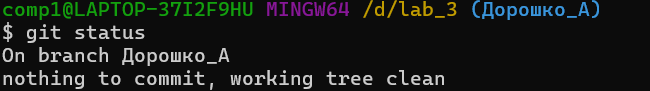
\includegraphics[width=8.5cm]{2.png}
    \caption{{\small A genetic algorithm scheme to search for the optimal neural
network architecture}}
 \end{figure}
 \begin{figure}[H]
    \centering
    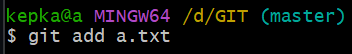
\includegraphics[width=8.5cm]{3.png}
    \caption{ {\small Neuroregulator synthesis algorithm scheme}\label{Figure3}}
 \end{figure}\vspace{-5pt}
 Simulation modeling allows for model validation after
training. Models of neuroregulators are saved to the
database for further use or additional training using
updated statistics.\par
The decision-making subsystem uses the constructed
models of neuroregulators.\par
Adaptation of the technological cycle control is carried
out on the basis of the operation of the constructed
neuroregulator, which forms corrective influences on the
process control system to prevent the range of changes
in the components Ufh of the control vector variables
Uh from going outside the allowed range.\par
Returning the values of control variables within the
acceptable intervals is carried out by means of special
adjustment means - initiating the launch of MTSO TP,
which change the values of the components of the set
of control variables Us or use equipment redundancy
schemes.\par
Provided that appropriate hardware and software interface tools are available, it is possible to implement
control adaptation in an automated mode, or to form a
recommendation system used by personnel servicing the
technological cycle.\par
Thus, when solving the problem of stabilizing the
parameters of technological operations in real time, multilevel mathematical models were used, including neural
network and simulation ones, and a new generation
hybrid intelligent computer adaptive control system was
implemented, created on the basis of open semantic
technologies for designing intelligent systems [7].
\begin{center}
\RomanNumeralCaps{6.} An example of a simulation model of a
probabilistic technological process control system
\end{center}\par
Simulation modeling of the interaction of control
system elements and components of a probabilistic technological process can be carried out on the basis of
synchronization schemes of their operation [7].\par 
Simulation modeling of the implementation of a
probabilistic technological process includes modeling of
microtechnological operations associated with resource
requests of a probabilistic nature, as well as possible
changes in control variables U, and the operation of
devices with possible device failures and their consequences.\par 
The initial parameters for constructing a control system simulation model (CS SM) of an probabilistic technical process (PTP) are a set of parameters characterizing
its composition and structure [7], including estimates of
the distributions of various parameters of the TP, collected during its operation observation using appropriate
software and hardware interface tools. In particular, these
include the number of implementations of the simulation
model N, the set Xi of PTP resource requests required
to run the executive elements of the control system, the
parameters of commutation of the executive elements
with synchronization elements, input signal generators
and the final operating element, configuration vector
of the equipment composition and a set of reliability
characteristics of the equipment.\par 
Simulation modeling of control system of TP is based
on the operation of a set of simulator units. Within
the framework of OSTIS technology, the solution to
the problem of operation of simulator units can be
formalized on the basis of a multi-agent approach [7],
when the SM of the PTP control system is implemented
as a set of agents corresponding to simulator units that
can exchange data through sc-texts.\par
Within the framework of the problem under consideration, the solver of the problem of operation of a simulator 
\end{multicols}
\end{document}





